%-----------------------------------------------------------------------------%
% \section{Data Buoys}
% %-----------------------------------------------------------------------------%
% Dikutip dari McLeod dan Ringwood (2022), data buoys dideskripsikan sebagai alat atau \textit{tools} untuk pemantauan laut di mana unit independen pelampung berskala kecil yang dilengkapi panel surya \textit{Photovoltaics} (PV). Panel ini menyediakan pasokan daya sehingga tidak memerlukan melakukan perawatan rutin dan dapat berfungsi secara otonom, menyediakan transmisi informasi periodik secara berkala, dan digunakan untuk prakiraan cuaca serta pemantauan iklim.

% Data buoys berkontribusi besar terhadap pemahaman ilmiah tentang lingkungan maritim, baik yang ditempatkan di dasar laut atau hanyut mengikuti arus, di atas permukaan laut atau di bawah permukaan laut dengan kedalaman meter tertentu. Pelampung dilengkapi berbagai jenis sensor tergantung pada target pemantauan yang akan diteliti, dan secara konstan mencatat serta mentransmisikan data secara dinamis yang mencakup parameter meteorologi, dinamika gelombang laut, arus, serta sifat fisik dan kimia air laut \parencite{mcleodringwood2022}.

% \textit{The Research Moored Array for African-Asian-Australian Monsoon Analysis and prediction} (RAMA) adalah sebuah jaringan yang dirancang untuk mempelajari variabilitas Samudera Hindia dan pengaruhnya terhadap pembalikan angin muson di kawasan Asia, Afrika, dan Australia untuk produksi pertanian, sehingga dapat mengisi kesenjangan data yang sebelumnya kurang terjangkau dibandingkan Samudra Pasifik dan Samudra Atlantik \parencite{mcphaden2009}. Di antara tiga samudra tropis, Samudra Hindia memiliki keunikan karena terhalang pada 25° LU oleh daratan Asia. Samudra Hindia menerima panas dari dua samudra tropis lainnya, yaitu Pasifik melalui Arus Lintas Indonesia (\textit{Indonesian Throughflow}) \parencite{arnold2001} dan menyalurkan panas ke Atlantik melalui Sistem Arus Agulhas (\textit{Agulhas Current System}) \parencite{rujiter1999}.
%-----------------------------------------------------------------------------%
\chapter{\babDua}
\thispagestyle{fancy}
%-----------------------------------------------------------------------------%
\section{Data BMKG}
Badan Meteorologi, Klimatologi, dan Geofisika (BMKG) adalah Lembaga Pemerintah Non-Kementrian (LPNK), bertanggung jawab untuk prediksi cuaca, pemantauan iklim, dan mitigasi bencana terkait kondisi atmosfer di Indonesia \parencite{sujalu2020}. Di bawah kepemimpinan seorang Kepala Badan, BMKG menjalankan peran strategis dalam penyediaan informasi meteorologi, klimatologi, kualitas udara, dan geofisika sesuai perundang-undangan yang berlaku \parencite{boy2020}. Sejak tahun 2017, 41 radar cuaca telah berhasil disebar di wilayah Indonesia dari Aceh hingga Papua \parencite{prakarsa2019}. Data cuaca hasil pengumpulan radar BMKG selanjutnya diproses dan disimpan ke dalam \textit{database}, memungkinkan otomasi pemrosesan data dan analisis pemodelan pola cuaca dapat dijalankan

\section{Data Satelit}
Citra Satelit Sentinel-2 merupakan bagian program Copernicus. Dikembangkan oleh European Space Agency (ESA) dan European Union (EU), menyediakan layanan citra satelit resolusi tinggi guna mendukung pemantauan tutupan lahan, perubahan iklim, dan mitigasi bencana. Konstelasi Sentinel-2 terdiri dari dua satelit, yaitu Sentinel-2A (diluncurkan 23 Juni 2015) dan Sentinel-2B (diluncurkan 7 Maret 2017), keduanya membawa instrumen pencitraan multispektral (MSI) dengan 13 saluran spektral mencakup cahaya tampak, \textit{near-infrared} (NIR), dan \textit{shortwave infra-red} (SWIR). Ketersediaan data secara \textit{open-source} memungkinkan negara berkembang dengan keterbatasan anggaran untuk mengakses data penginderaan jauh \parencite{phiri2020}.

Data Sentinel-2 memiliki karakteristik instrumen multispektral maupun multitemporal, sehingga mendukung penerapan analisis data menggunakan algoritma \textit{mechine learning}. Beberapa algoritma di antaranya \textit{Support Vector Machine} (SVM), \textit{Random Forest} (RF), \textit{Extreme Gradient Boosting} (XGBoost), dan \textit{Deep Learning}. Keunggulan saluran \textit{red edge} sebesar 25\% dan \textit{shortwave infrared} sebesar 23\% dari Sentinel-2 terbukti meningkatkan akurasi klasifikasi tutupan lahan signifikan, terutama ketika menggunakan citra multitemporal yang merepresentasikan kondisi musim yang berbeda. Integrasi pendekatan \textit{machine learning} dengan metode \textit{smoothing} pada tahap \textit{preprocessing} dapat meningkatkan kualitas data, hasil analisis iklim menjadi lebih reliabel untuk pemodelan \parencite{abdi2020}

\section{Data NASA POWER}
NASA \textit{Prediction of Worldwide Energy Resources} (POWER) merupakan layanan data iklim dan meteorologi global berbasis observasi satelit yang dikembangkan oleh \textit{National Aeronautics and Space Administration} (NASA). Layanan ini menyediakan data harian variabel suhu, radiasi matahari, kelembapan, curah hujan, dan kecepatan angin, agar mendukung wilayah dengan keterbatasan stasiun cuaca darat \parencite{rodrigues2021}.

NASA POWER juga memiliki kemudahan dalam mengintegrasikan data, karena memiliki API untuk mengakses data dari server NASA tanpa melakukan unduh manual. API memungkinkan proses pengolahan data menjadi lebih konsisten, dan terotomatisasi, sehingga sangat mendukung pembangunan sistem yang membutuhkan data iklim secara \textit{real-time} maupun historis. NASA POWER tidak hanya menyediakan data yang lengkap, namun juga mempermudah penggunaannya dalam berbagai aplikasi penelitian, analisis, serta pengembangan sistem otomasi \parencite{sparks2018}.

\section{Metode \textit{Smoothing}}
Metode \textit{smoothing} termasuk ke dalam pengolahan data yang melibatkan peramalan urutan nilai dan menunjukkan tren dari sekumpulan data berfluktuasi acak \parencite{castillo2022}. Teknik ini digunakan untuk mengisi data hilang atau meredam fluktuasi dalam dataset sehingga menghasilkan data yang \textit{clean}. \textit{Single Exponential Smoothing} bergerak dengan pembobotan canggih namun tetap mudah digunakan, sehingga hanya cocok untuk data historikal dan tidak mampu menangkap tren serta pola musiman \parencite{susanto2017}.

Untuk mengatasi keterbatasan tersebut, diperlukan pendekatan lebih komprehensif, Holt-Winters (HW) \textit{Exponential Smoothing} atau \textit{Triple Exponential Smoothing}. Holt-Winters merupakan perluasan teknik \textit{smoothing} dengan mengintegrasikan tiga komponen utama, yaitu level (α), tren (γ), dan musiman (δ) \parencite{trull2020}. HW secara rekursif memperbarui nilai dasar, perubahan jangka panjang, serta pola berulang tahunan dalam data.

Di sisi lain, pengembangan metode \textit{Long Short-Term Memory} (LSTM) menunjukkan hasil menjanjikan dalam peramalan hidrologi, dengan meningkatkan akurasi prediksi. \textit{Smooth}-LSTM menggabungkan arsitektur LSTM dengan teknik \textit{smoothing} untuk menghilangkan fluktuasi acak dalam data sekuensial, memungkinkan model menangkap pola temporal lebih kompleks dan menghasilkan prediksi akurat \parencite{khatun2023}.

\section{DBMS}
\textit{Database Management System} (DBMS), merupakan sebuah \textit{software tools} dalam masalah mengorganisasikan data dan menyajikan akses untuk program aplikasi. DBMS berperan sebagai \textit{interface} dan file fisik, sehingga mempermudah programmer dalam memahami struktur penyimpanan data \parencite{susanto2019}. DBMS ditujukan untuk menyediakan keamanan data, pembagian data, dan konsistensi hasil dari analisis yang diinginkan untuk ketepatan pengambilan keputusan \parencite{sabrina2023}.

DBMS dapat memodelkan \textit{Entity Relationship Diagram} (ERD) memakai \textit{Structured Query Language} (SQL) \parencite{hoffman2001}. Operasional DBMS memastikan bahwa transaksi data berlangsung konsisten melalui prinsip ACID (\textit{Atomicity, Consistency, Isolation, and Durability}). Namun, subjek kinerja dari optimasi SQL untuk skala besar perusahaan, \textit{parallel databases}, dan \textit{big data} akan tidak efektif dan dapat menghasilkan \textit{resources} sistem dan server, yang menyebabkan penguncian \textit{database} dan masalah kehilangan data \parencite{khan2022}. Seiring dengan meningkatnya skala data dan kebutuhan akan performa tinggi dalam DBMS, NoSQL hadir sebagai alternatif untuk mengatasi keterbatasan dari SQL. NoSQL memiliki hasil waktu \textit{query execution} lebih cepat jika dibandingkan dengan SQL, hal ini dipengaruhi fakta bahwa semua informasi disimpan dalam satu dokumen, berbeda dengan SQL yang disimpan dalam beberapa tabel berelasi melalui penggunaan JOIN. NoSQL memiliki kerja dalam Operasi CRUD, yang mempengaruhi kemampuan transaksi ACID serta skabilitas lebik baik \parencite{rade2022}.

\begin{table}[H]
    \centering
    \caption{Perbandingan SQL dan NoSQL berdasarkan karakteristik}
    \label{tab:sql_vs_nosql}
    \begin{tabular}{|l|p{5cm}|p{4cm}|}
        \hline
        \textbf{Karakteristik} & \textbf{SQL (Relasional Database)} & \textbf{NoSQL (Non-Relasional Database)} \\
        \hline
        Struktur Data & Tabel dengan baris dan kolom. & Berbagai format \textit{key-value}, \textit{document}. \\
        \hline
        Skema & Skema tetap dan harus didefinisikan sebelum data disimpan. & Tidak memiliki skema tetap, lebih fleksibel dalam menyimpan data. \\
        \hline
        \textit{Query Language} & \textit{SQL (Structured Query Language)} untuk manipulasi data. & Tergantung bahasa kueri pada tipe NoSQL (misalnya, MongoDB \textit{Query Language}, CQL untuk Cassandra). \\
        \hline
        Skalabilitas & Vertikal – Memerlukan peningkatan spesifikasi server (CPU, RAM, storage). & Horizontal – Skalabilitas \textit{sharding} dan \textit{distributed computing}. \\
        \hline
        Kecepatan \textit{Query} & Lambat jika kueri kompleks karena menggunakan \textit{JOIN}. & Cepat karena tidak menggunakan \textit{JOIN}. \\
        \hline
        Tipe Data & Cocok untuk data terstruktur. & Cocok untuk data semi-terstruktur dan tidak terstruktur. \\
        \hline
    \end{tabular}
\end{table}

\section{Next.js}
Dari balik layar, Next.js juga mengabstraksi dan secara otomatis dan mengonfigurasi \textit{configuration} yang diperlukan untuk React, termasuk \textit{bundling}, \textit{compiling}, dan banyak lagi. Hal ini memungkinkan pengguna untuk fokus membangun aplikasi daripada menghabiskan waktu dengan konfigurasi \parencite{nextjsdoc2025}.

Keunggulan lainnya adalah fleksibilitas dalam kustomisasi yang memungkinkan pengguna menyesuaikan parameter aplikasi sesuai kebutuhan. Struktur komponen yang modular juga mempermudah pengembangan fitur baru tanpa mengubah struktur utama aplikasi. Dalam hal manajemen data, Next.js menggunakan API \textit{routes} untuk memastikan sinkronisasi data \textit{real-time} serta menjaga integritas data dengan validasi yang ketat.

\section{REST API}
\textit{Representational State Transfer Application Programming Interface} (REST API) digambarkan sebagai arsitektur layanan web yang memungkinkan komunikasi antara klien dan server menggunakan standar protokol HTTP (\textit{Hypertext Transfer Protocol}). REST API dikembangkan sebagai solusi untuk menyediakan antarmuka yang ringan, fleksibel, dan mudah diimplementasikan dalam berbagai platform. Salah satu faktor utama yang menjadikannya standar dalam pengembangan aplikasi web adalah penggunaan format data  JSON, XML dan HTML yang  mudah dibaca dibandingkan format API lainnya \parencite{banias2021}.
\begin{figure}
    \centering
    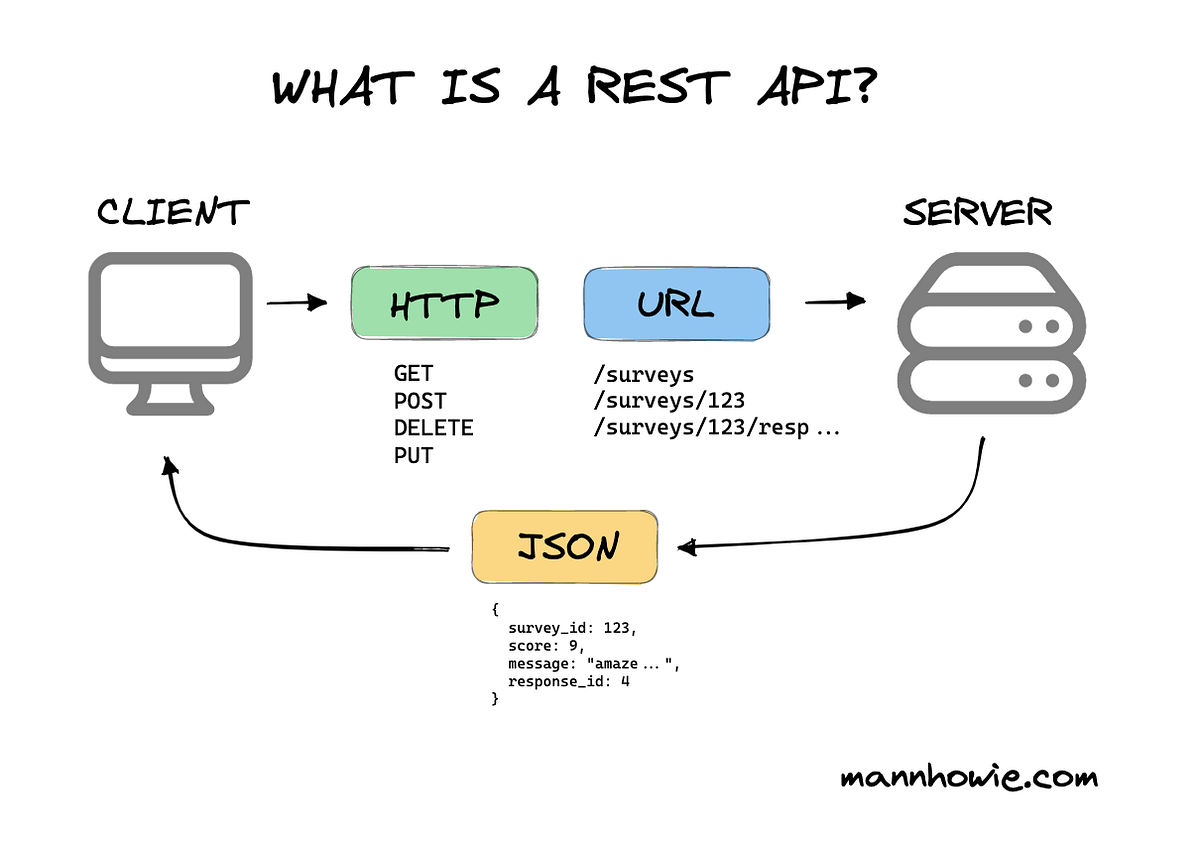
\includegraphics[width=0.80\linewidth]{assets//pics/rest_api.png}
    \caption{Alur REST API}
    \label{fig:enter-label}
\end{figure}
Dalam aspek keamanan, REST API kini banyak menggunakan OAuth 2.0 dan JWT (JSON Web Token) untuk autentikasi guna mencegah serangan keamanan \textit{man-in-the-middle}. Implementasi fitur \textit{caching} dan \textit{rate limiting} telah meningkatkan efisiensi REST API dengan mempercepat respons dan mengurangi beban server. Suatu \textit{request} dapat dianggap dibentuk oleh \textit{endpoint} REST API, metode API-yang sebagian besar mencakup operasi CRUD (\textit{GET, PUT, POST, DELETE}) dan parameter. Adapun \textit{status code} mewakili jenis \textit{response} yang diterima dari REST API berbasis HTTP, dengan kode memiliki 3 digit. Digit pertama adalah kategori dengan terbagi menjadi 5 jenis kode, diantaranya yaitu 1xx (proses informasi), 2xx (ok), 3xx (\textit{redirect}), 4xx (\textit{client error}), dan 5xx (\textit{server error}). Digit kedua dan ketiga menunjukkan \textit{status code} dalam rentang digit pertama. IANA (\textit{Internet Assigned Numbers Authority}) mengelola lebih dari 40 kode HTTP resmi \parencite{fitri2022}.

\section{Hono.js}
Hono.js merupakan \textit{web framework} yang dikembangkan untuk membantu mengembangkan aplikasi web dan API yang lebih cocok dengan tren saat ini, di mana efisiensi dan ringannya suatu API sangat diperhitungkan. Hono.js dikembangkan dalam bahasa Typescript, memiliki performa tinggi dan kompatibel untuk \textit{multiplatform}, bahkan \textit{environtment} yang bersifat \textit{serverless}, misalnya Deno, Fastly Compute, Lambda@Edge, Bun, Vercel, AWS Lambda, dan Node.js \parencite{honojs2021}.

Keunggulan utama Hono.js terletak pada kinerjanya yang tinggi serta kemampuannya untuk berjalan di berbagai \textit{runtime}, memberikan fleksibilitas yang besar dalam pengembangan aplikasi modern. Adapun penggunaan sintaks yang mirip dengan Express.js juga membuatnya mudah dipelajari bagi pengembang yang sudah terbiasa dengan ekosistem JavaScript. Namun, dibandingkan dengan \textit{framework} populer  Express.js atau Next.js, ekosistem Hono.js masih dalam tahap perkembangan dengan sumber daya dan komunitas yang lebih terbatas. Meski ekosistemnya masih berkembang, Hono.js mulai mendapatkan perhatian karena kemampuannya dalam membangun aplikasi web yang ringan, responsif, dan mudah di-\textit{deploy}.

\section{Agile}
Metode pengembangan perangkat lunak berbasis Agile adalah metode yang berfokus pada fleksibilitas, iterasi cepat, kolaborasi tim, dan respon terhadap perubahan. Metode ini menggantikan metode Waterfall karena sifatnya kaku terhadap perubahan, Agile muncul sebagai respons terhadap kebutuhan industri yang mengarah dinamis dan penuh perubahan. Sejak diperkenalkannya Agile Manifesto pada tahun 2001, metode Agile semakin banyak diadopsi di industri karena memberikan kecepatan dalam pengembangan, kepuasan pelanggan, dan peningkatan kualitas. \parencite{jovanovic2020}.

\begin{figure}
    \centering
    
\includegraphics[width=0.75\linewidth]{assets//pics/agile_framework.jpg}
    \caption{Agile \textit{Framework}}
    \label{fig:enter-label}
\end{figure}

Agile \textit{Framework} memiliki beberapa komponen utama yang mendukung efektivitasnya dalam pengembangan perangkat lunak dan manajemen proses bisnis. \textit{Iterative Development} menjadi salah satu prinsip dasar, yang menekankan pada pengiriman perubahan kecil dan bertahap dibandingkan merilis produk secara keseluruhan. Pendekatan ini memungkinkan umpan balik berkelanjutan dan peningkatan kualitas produk secara iteratif. 

Dari segi adaptabilitas, tim memungkinkan untuk beradaptasi dengan cepat terhadap perubahan ruang lingkup proyek. Dalam konteks \textit{Business Process Management} (BPM), Agile mengintegrasikan berbagai komponen yang mendukung ketangkasan bisnis, termasuk pemanfaatan teknologi  \textit{process mining} untuk meningkatkan respons organisasi terhadap perubahan. Sehingga dapat dikatakan Agile tidak hanya meningkatkan efisiensi pengembangan perangkat lunak tetapi juga membantu organisasi menjadi lebih fleksibel dan inovatif dalam mengelola proses bisnis \parencite{badakhshan2019}.

\section{Penelitian Terkait}
Penelitian terkait pernah dilakukan oleh para peneliti sebelumnya dengan tujuan menambah wawasan terkait metode penelitian yang akan digunakan nantinya. Penelitian terkait juga bermanfaat dalam membandingkan tema penelitian yang sudah ada, atau metode apa yang membedakan penelitian \saya{}  yang dijabarkan dalam tabel di bawah ini.

\renewcommand{\arraystretch}{1.5} 
\begin{longtable}{|p{0.05\textwidth}|p{0.25\textwidth}|p{0.35\textwidth}|p{0.25\textwidth}|}
\caption{Penelitian terkait} \label{tab:penelitian_terkait} \\
\hline
\textbf{No.} & \textbf{Judul Penelitian} & \textbf{Fokus Utama} & \textbf{Perbedaan} \\ \hline
\endfirsthead
\hline
\textbf{No.} & \textbf{Judul Penelitian} & \textbf{Fokus Utama} & \textbf{Perbedaan} \\ \hline
\endhead
\hline
\endfoot
\hline
\endlastfoot
1 & \textit{Performance of Smoothing Methods for Reconstructing} NDVI \textit{Time-Series and Estimating Vegetation Phenology from} MODIS \textit{Data} \parencite{cai2017} & 
Evaluasi kinerja berbagai metode \textit{smoothing} untuk rekonstruksi NDVI \textit{time-series} dari data MODIS untuk mengekstrak parameter fenologi vegetasi. Studi membandingkan lima metode Savitzky-Golay, LOESS, \textit{spline smoothing}, \textit{Asymmetric Gaussian}, dan \textit{Double logistic}
menggunakan data referensi lapangan serta data elevasi sebagai indikator variabilitas fenologi. & 
Evaluasi data satelit NDVI \textit{time-series} untuk menentukan metode \textit{smoothing} terbaik, namun tidak tersedia untuk data sumber lain data BMKG, dan NASA Power. \\ \hline
2 & \textit{Implementation of a Web based Weather Monitoring Station and Data Storage System} \parencite{cesar2019} & Implementasi web \textit{Automated Weather Station} (AWS) untuk memantau kondisi cuaca otomatis di Science Garden, PAGASA, Filipina. Menggantikan metode pengamat pergi ke lapangan, sehingga mengurangi kesalahan pengukuran akibat faktor pada kondisi cuaca ekstrem. & 
Berfokus pada penggunaaan sistem \textit{Automated Weather Station} (AWS) dan modul GSM, namun hanya berfokus pada data cuaca. Peneliti mengkalibarasi sensor di PAGASA berkala, sedangkan \saya{} mempersiapkan data yang tersedia dari \textit{platform}, tanpa melibatkan sensor dan modul. \\ \hline
3 & Antisipasi Terjadinya Pemanasan Global Dengan Deteksi Dini Suhu Permukaan Air Menggunakan Data Satelit \parencite{mulyani2021} & Deteksi dini SPL menggunakan data satelit sebagai upaya mengantisipasi pemanasan global. SPL merupakan indikator penting dalam dinamika iklim global, di mana peningkatannya dapat menyebabkan perubahan iklim ekstrem. SPL dapat dipantau secara spasial dan temporal, memungkinkan analisis tren perubahan suhu selama 32 tahun perairan Indonesia. & Penelitian ini berfokus pada anomali SPL sebagai indikator penting dalam menganalisis tren perubahan suhu, menggunakan data \textit{Moderate Resolution Imaging Spectroradiometer} (MODIS), sedangkan \saya{} menggunakan data NDVI, EVI, dan LSWI dari Google Earth Engine. \\ \hline

4 & Perubahan Iklim Di DAS Krueng Aceh \parencite{safitri2023} & Analisis tren perubahan iklim di DAS Krueng Aceh selama periode 2001–2020 melalui pengamatan tren menggunakan klasifikasi Schmidt–Ferguson. Adanya peningkatan curah hujan signifikan di dua stasiun pengamatan (BMKG Indrapuri dan BMKG Blang Bintang) serta tren kenaikan suhu udara, yang berdampak pada pergeseran tipe iklim dari kategori C (agak basah) ke B (basah). & Berfokus pada tren curah hujan dan suhu udara menggunakan 2 data stasiun BMKG Indrapuri dan Blang Bintang, namun tidak mengimplementasikan sistem data iklim secara otomatis, sehingga pengamatan data tidak dinamis dan hanya mengandalkan data historikal. \\ \hline
\end{longtable}

\vspace*{0.8cm} 
